\documentclass[12pt]{Article}

% Package to handle graphics inclusion (optional)
\usepackage{graphicx}
% Package for better math formatting (optional)
\usepackage{amsmath}
% For references (optional)
\usepackage{cite}
% Package to customize title position
\usepackage{titling}
\usepackage{subcaption}
\usepackage{listings}
\usepackage{xcolor}
\usepackage{hyperref}
\usepackage{float}

\lstset{
    language=Python,
    basicstyle=\ttfamily\small,
    keywordstyle=\color{blue},
    commentstyle=\color{gray},
    stringstyle=\color{red},
    showstringspaces=false,
    numbers=left,
    numberstyle=\tiny\color{gray},
    breaklines=true,
    frame=single,
    captionpos=b
}


\usepackage{silence}
\usepackage{wrapfig}
\usepackage{float}
\usepackage{adjustbox}
\usepackage[margin=0.8in]{geometry}  % Adjust the margin as needed

\setlength{\parindent}{15pt} 
% Adjust the title position
\setlength{\droptitle}{-6em}% Adjust the value as needed
% Title and Author information
\title{Final Report - Messaging App}
\author{
    Hugo Garrido-Lestache
}
\date{\today \\ CSC 5201 301}

\begin{document}

\maketitle
\section*{Introduction}
For my Final Project, I created a messaging app that allowed users to send messages to each other.
This app was a web app with the abilities to send direct messages, group messages and create group chats.
It also handled users login and registration.
I thought this service could be a fun project to practice my skills, 
which could then be used to message my friends and family.
This service was designed to be similar to messaging apps such as WhatsApp or Microsoft Teams.

\section{Use cases}
The application was developed to support the following use cases, many of which were only thought about after the initial implementation.

\begin{itemize}
    \item User login and registration - Users needed to be able to login and register to use the app.
    \item User logout - Users needed to be able to logout of the app.
    \item List all users - Users needed to be able to see a list of all users.
    \item List all messages - Users needed to be able to see a list of all recent messages.
    \item Send direct messages to other users - Users needed to be able to send direct messages to other users.
    \item Create group chats - Users needed to be able to create group chats.
    \item Send messages to group chats - Users needed to be able to send messages to group chats.
    \item Add users to group chats - Users needed to be able to add users to group chats.
    \item Remove users from group chats - Users needed to be able to remove users from group chats.
\end{itemize}

\section{Business context \& Services}
Our business was separated into 3 services:

\begin{itemize}
    \item User service - This service was responsible for handling the user login and registration. It was responsible for managing the data on users in the database and ensuring that the users were authenticated.
    \item Message service - This service was responsible for handling the messages. It was responsible for managing the data on messages in the database and ensuring that the messages were stored and retrieved correctly.
    \item Group chat service - This service was responsible for handling the group chats. It was responsible for managing the data on group chats in the database and ensuring that the group chats were stored and retrieved correctly.
\end{itemize}

\section{Technical Implementation}
The backend of the messaging application leverages three Python-Flask microservices with MySQL databases:

\begin{itemize}
    \item \textbf{User Service}: Manages a \texttt{users} table with user credentials and profile information. Handles authentication, registration, and user profile queries.
    
    \item \textbf{Message Service}: Maintains two tables: \texttt{messages} for direct messaging and \texttt{group\_messages} for group communications. Stores message content, sender/recipient IDs, and timestamps.
    
    \item \textbf{Group Chat Service}: Controls the \texttt{groups} table containing group metadata, including name, creator, and a JSON array of member IDs.
\end{itemize}

\noindent Inter-service communication occurs via direct API calls. An example of this is that when displaying conversations, the Message Service queries its database for message content but calls the User Service to retrieve usernames. Similarly, the Group Chat Service validates members by checking with the User Service.
The application is deployed using Kubernetes and docker containers, this allowed me to deploy the application in a single node cluster.
A future enhancement would be implementing message queues between services to improve comunication between them, when at a larger scale such that each service can have multiple instances.
Please see the link to the repo for the code.

\section{What I Delivered}
I managed to implement all the services and endpoints to match the use cases.
I realized that I had to implement extra endpoints to deal with handling the cookies and sessions when in the web app.
I also realized that I had to implement endpoints to get user info, for the other services to use.
Throughout creating this I settled on less traditional design of having two ways of sending messages of direct and group messages.
These each had their own sections in the frontend and own endpoints, this separation helped me to implement the services easier but was not ideal.

Below are some screenshots of the app in action:

\begin{figure}[H]
    \centering
    \begin{subfigure}{0.45\textwidth}
        \centering
        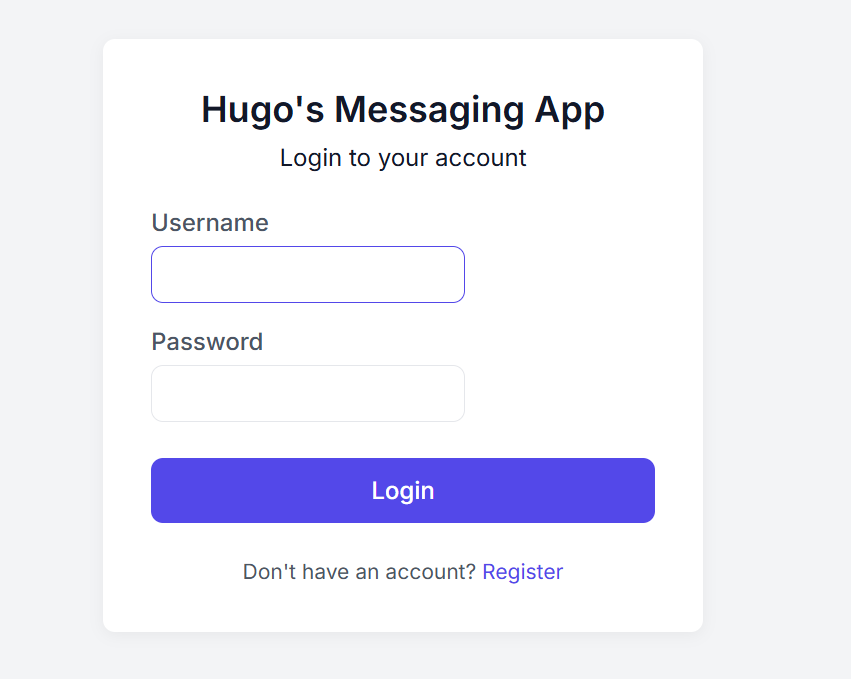
\includegraphics[width=\textwidth]{images/1.png}
        \caption{User login}
    \end{subfigure}
    \begin{subfigure}{0.45\textwidth}
        \centering
        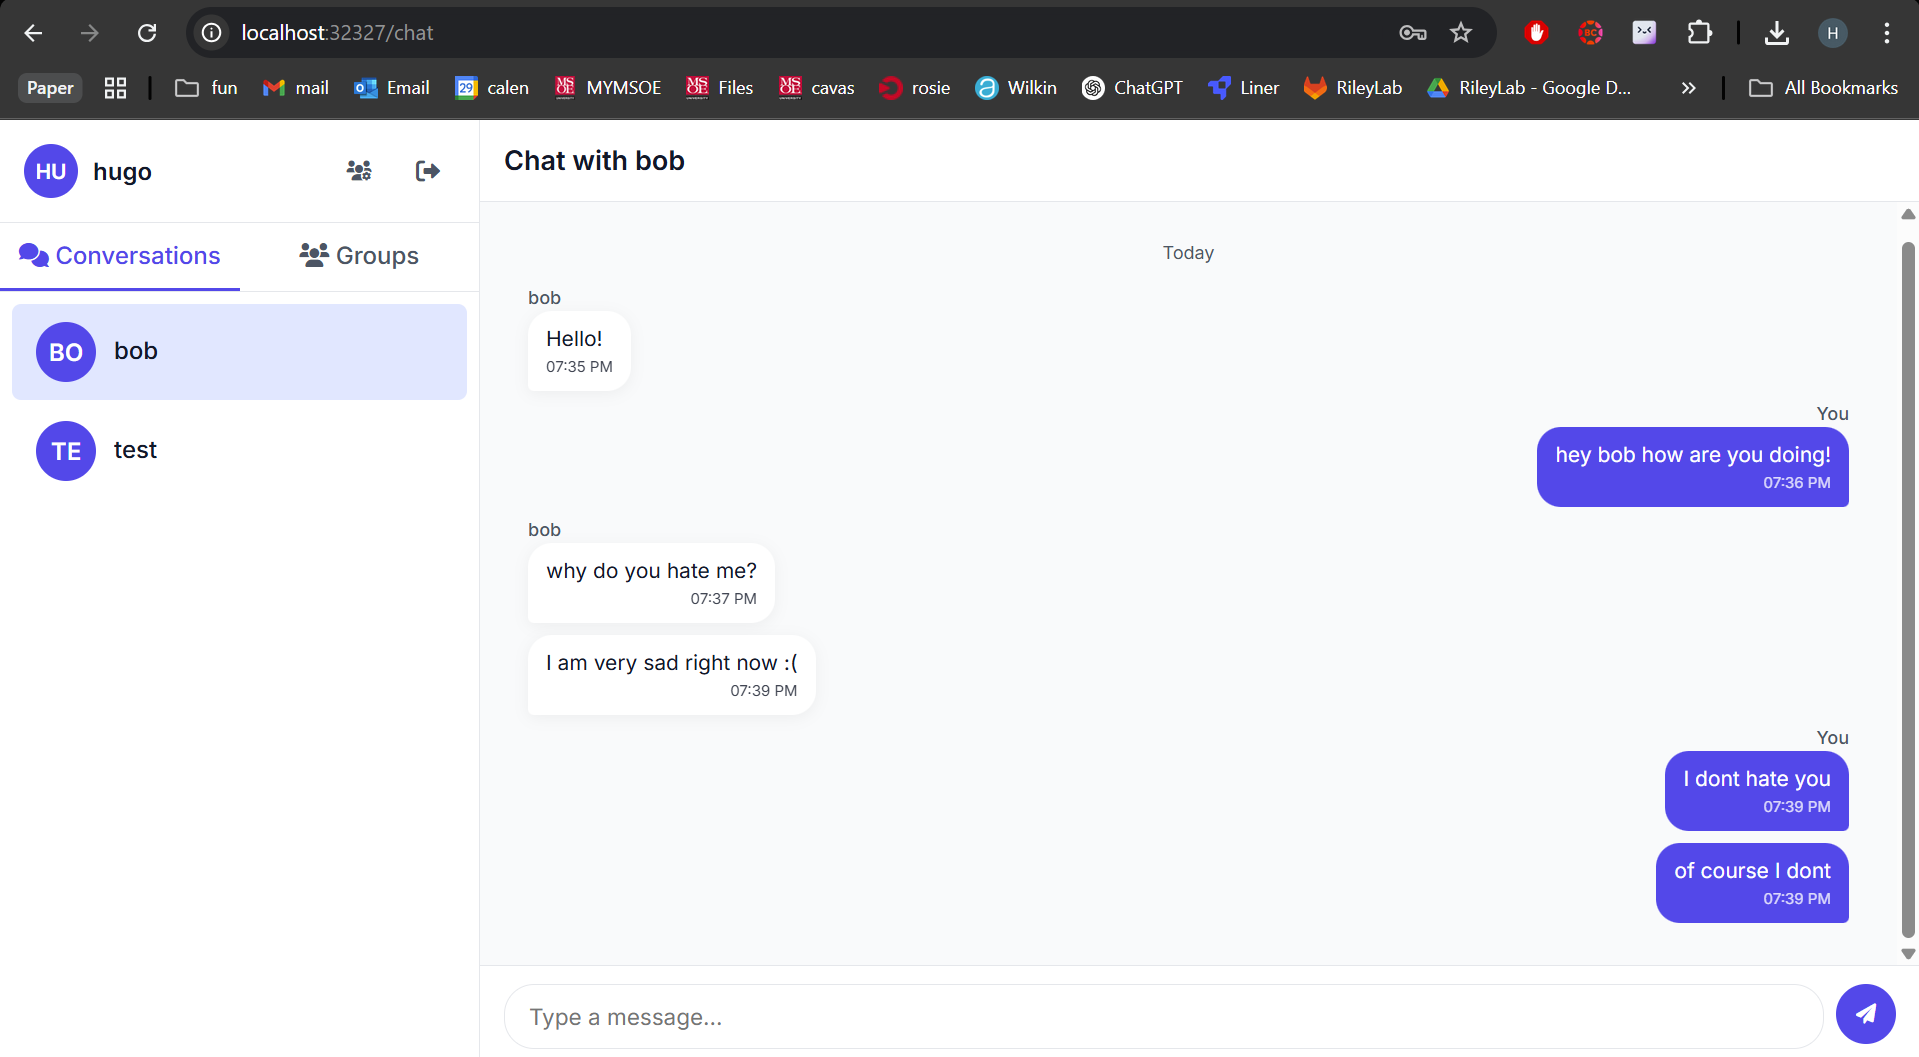
\includegraphics[width=\textwidth]{images/2.png}
        \caption{Direct message + Home page}
    \end{subfigure}
    \begin{subfigure}{0.45\textwidth}
        \centering
        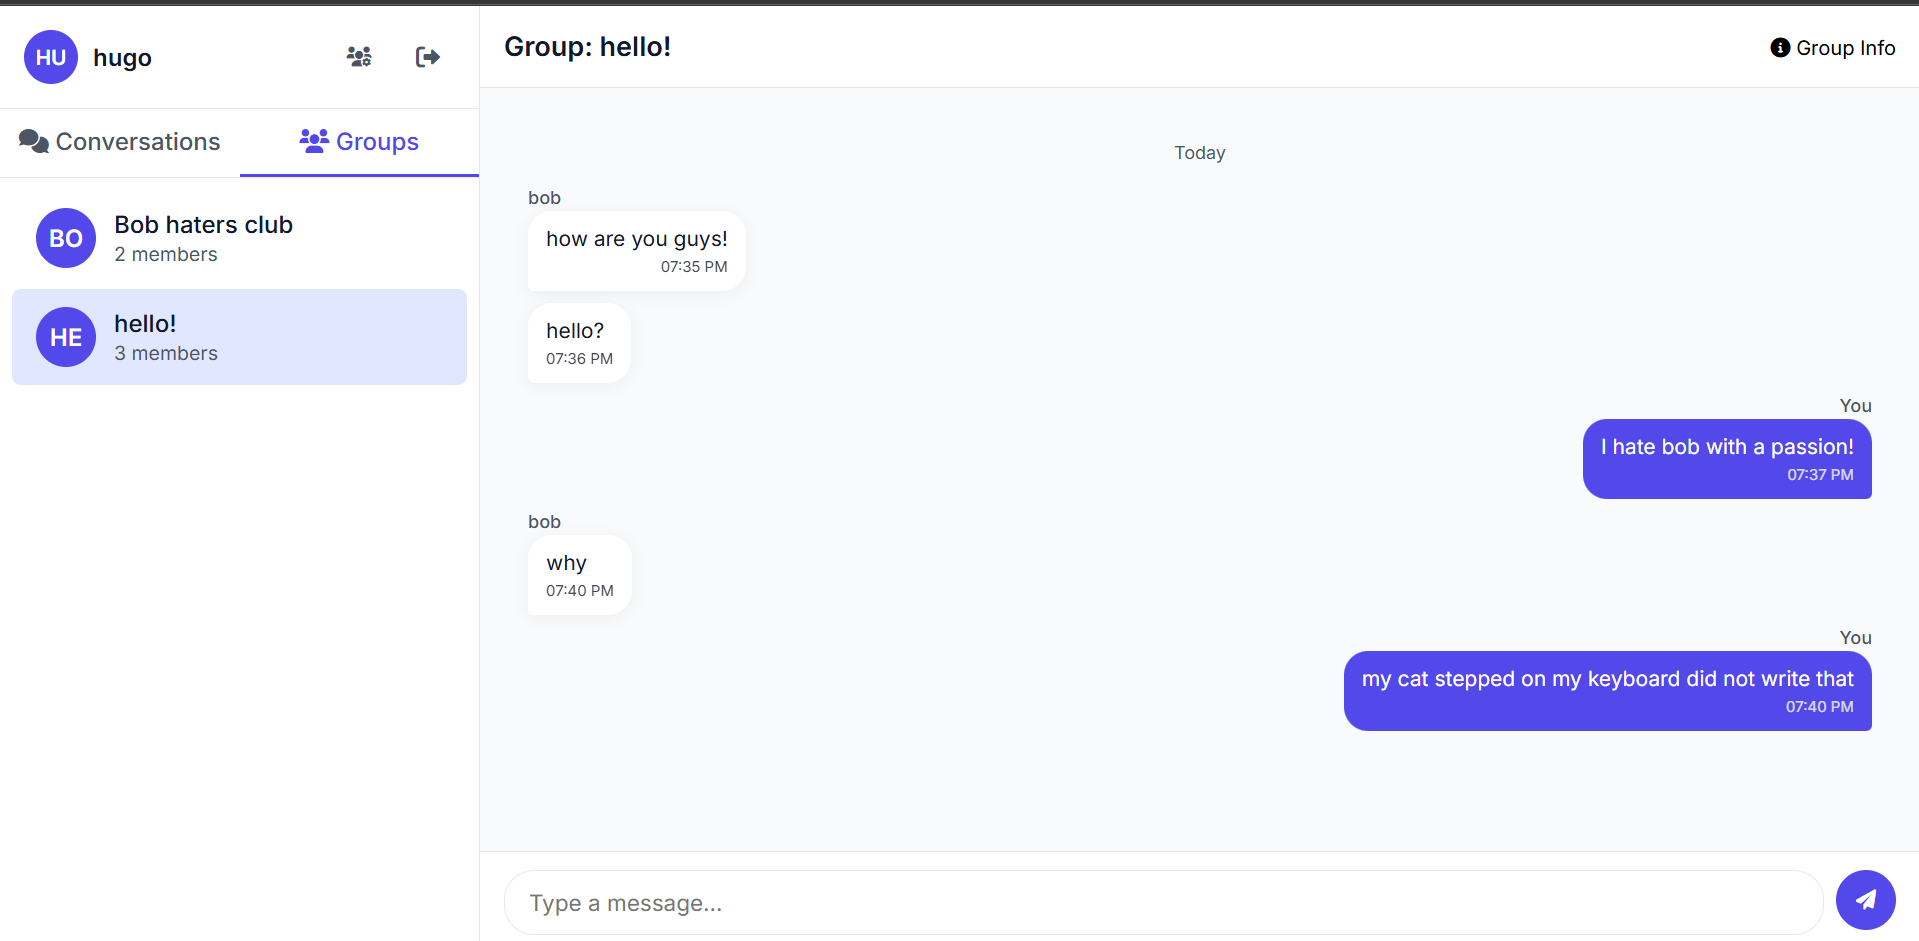
\includegraphics[width=\textwidth]{images/3.png}
        \caption{Group chat + Home page}
    \end{subfigure}
    \begin{subfigure}{0.45\textwidth}
        \centering
        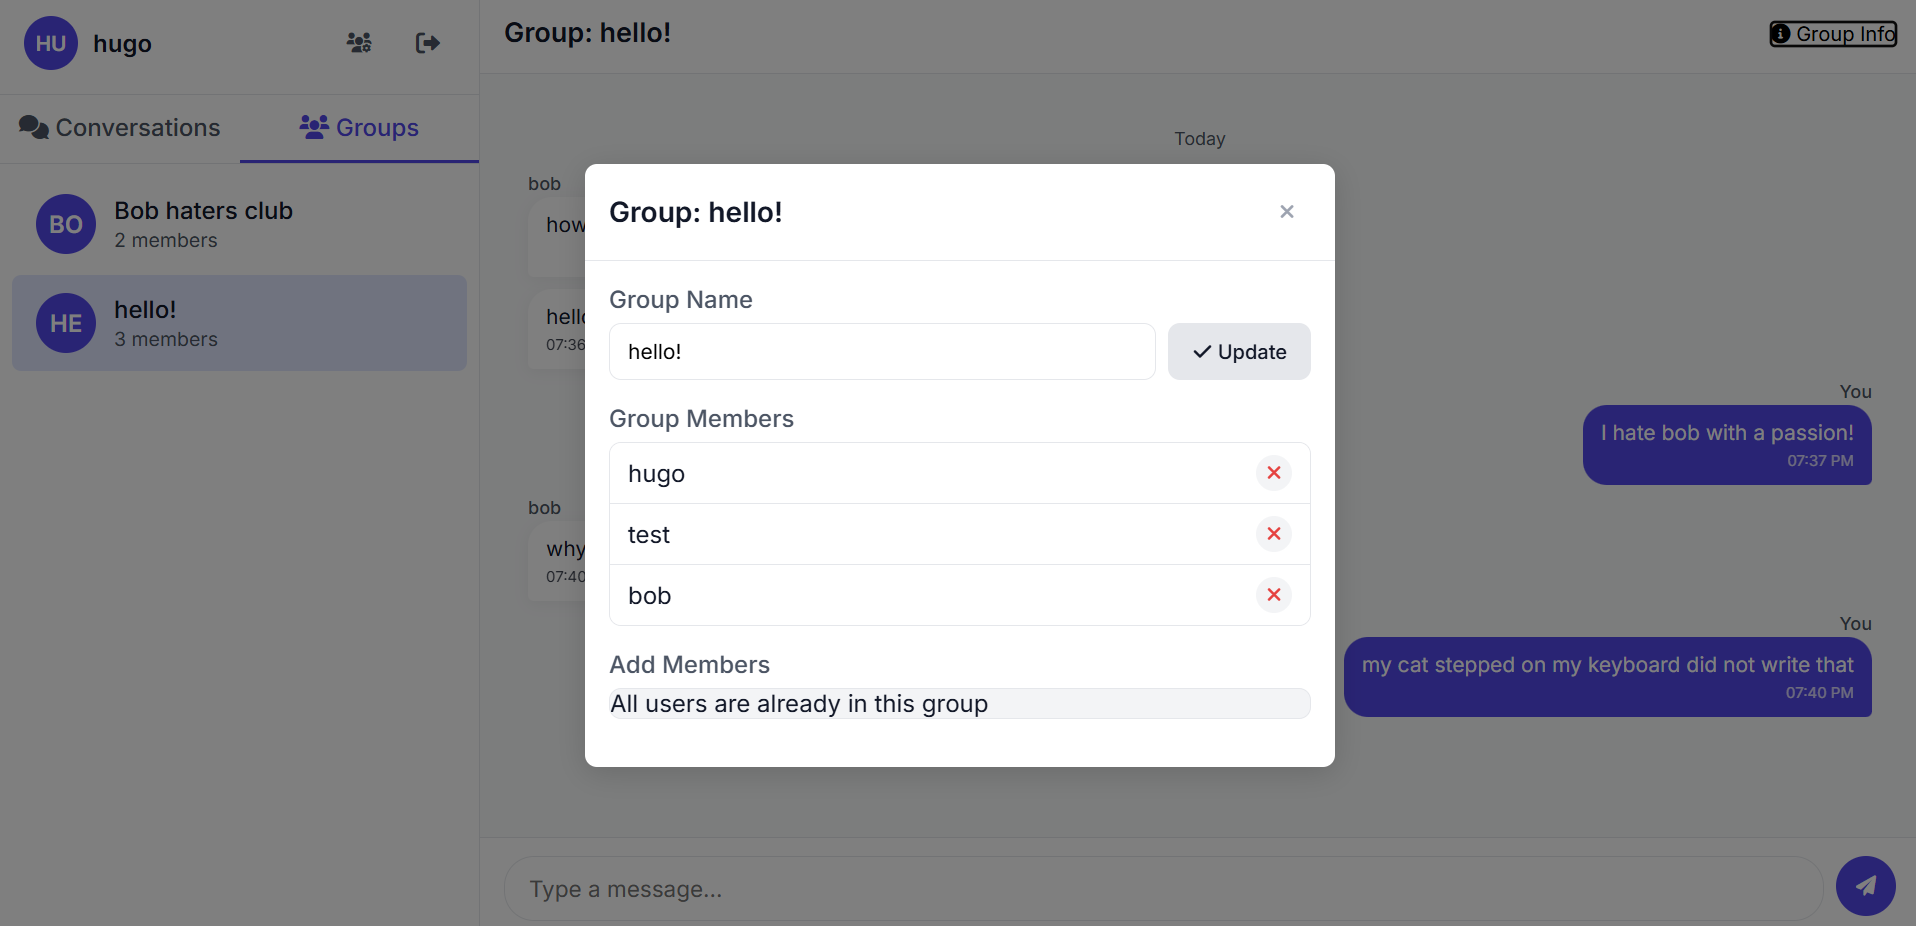
\includegraphics[width=\textwidth]{images/4.png}
        \caption{Group chat + edit group chat}
    \end{subfigure}
\end{figure}


\section{What I Learnt}
I learnt a lot about working with Docker and managing an application with multiple services.
Ensuring that the services were able to communicate with each other was challenging (passing their own services as a parameter to the other services).
It was intresting having them all work together to complete the overall goal.

I also learnt a lot about Kubernetes and how to deploy an application with it.
It was intresting to think abou the common data issue and having to replace that with inter-service communication.


\section{What I would do if I had more time}
I would not do much different, as in the end this project was more for fun and practice.
If I wanted to get this project to a more useable state, there would be many features I would add.
Such as security features, such as password hashing, testing scalability, and adding more features.
I would also want to be able to add the ability to send files and images, and also add a media service to store them.
Handeling notifications would also be a feature I would add, so users could know when they had a new message.

However if I had more time, I would likely work on a different project, as developing a messaging app is not very usefull which so many other services already providing this.
I would want to create something more novel.

\section{Conclusion}
In conclusion, I enjoyed working on this project and it was a fun way to practice my skills.
And I think I have learnt a lot from it.
Goodbye!

\section{Link to repo}
\href{https://github.com/Hugogales/microservices-final-project}{Link to repo}



\href{https://github.com/Hugogales/microservices-final-project}{https://github.com/Hugogales/microservices-final-project}



\end{document}
